\chapter{Le quark top au LHC : production et nouvelle physique}

\begin{fmffile}{chapitre5}

Le top quark est la particule élémentaire la plus lourde connu à ce jour. De part ses propriétés, il est attendu que le top quark joue un rôle spécial dans la découverte de physique au-delà du Modèle Standard. En effet, on verra par la suite que de nombreux modèle prédisent de nouvelles particules se couplant préférentiellement au quark top. Avant de détailler ces modèles, il est intéressant de passer en revue les propriétés du quark top.

\bigskip

Le top quark a été découvert en 1995 par les expériences D0 et CDF au Tevatron. Son existence était cependant prédite bien avant son observation. En effet, le quark $b$, découvert en 1977, se désintègrent par interaction faible, désintégration autorisée uniquement lorsque la particule appartient à un doublet de $SU(2)_L$, ce qui implique qu'un partenaire d'isospin du quark $b$ doit exister. On présente ci-dessous les différents modes de production du quark top, ainsi que ses modes de désintégrations. Un résumé de ses propriété sera aussi détaillé.

\section{Production du top quark}

\subsection{Production par paires}

Le mécanisme de production dominant des quarks top en collisionneur hadronique est \emph{via} interaction forte. Comme cette interaction conserve la saveur, le quark top doit donc être produit par paire. Environ \SI{80}{\%} de cette production intervient par fusion de gluons, et \SI{20}{\%} par annihilation de quarks. De récent progrès ont été fait dans le calcul de la section efficace de production de paire \ttbar, connu maintenant de façon exact au NNLO (\emph{next-to-next-to-leading order}) \citep{Czakon:2013goa}. Au LHC, pour $\sqrt{s} = \SI{8}{\TeV}$, on a $\sigma_{\ttbar} = \SI{245.8}{\pb}$. On présente \cref{fig:ttbar_diagrams} les diagrammes de Feynman des différents modes de production de paires \ttbar.

\begin{figure}[tbp] \centering
    \subcaptionbox{\label{fig:ttbar_fusion_gluon_1}}[0.32\textwidth]{
    \begin{fmfgraph*}(120,60)
        \fmfpen{0.5}
        \fmfleft{i1,i2}
        \fmfright{o1,o2}
        \fmf{gluon}{i1,v1,i2}
        \fmf{gluon}{v1,v2}
        \fmf{fermion}{o1,v2,o2}
        \fmfdot{v1,v2}
        \fmflabel{$t$}{o2}
        \fmflabel{$\bar{t}$}{o1}
    \end{fmfgraph*}
    }\hfill
    \subcaptionbox{\label{fig:ttbar_fusion_gluon_2}}[0.32\textwidth]{
    \begin{fmfgraph*}(140,60)
        \fmfpen{0.5}
        \fmfleft{i1,i2}
        \fmfright{o1,o2}
        \fmf{gluon}{i1,v1}
        \fmf{gluon}{i2,v2}
        \fmf{fermion}{o1,v1}
        \fmf{fermion}{v2,o2}
        \fmf{fermion,tension=1}{v1,v2}
        \fmfdot{v1,v2}
        \fmflabel{$t$}{o2}
        \fmflabel{$\bar{t}$}{o1}
    \end{fmfgraph*}
    } \hfill
    \subcaptionbox{\label{fig:ttbar_qq}}[0.32\textwidth]{
    \begin{fmfgraph*}(120,60)
        \fmfpen{0.5}
        \fmfleft{i1,i2}
        \fmfright{o1,o2}
        \fmf{fermion}{i1,v1,i2}
        \fmf{gluon}{v1,v2}
        \fmf{fermion}{o1,v2,o2}
        \fmfdot{v1,v2}
        \fmflabel{$t$}{o2}
        \fmflabel{$\bar{t}$}{o1}
    \end{fmfgraph*}
    }\hfill
    \caption{Diagrammes de Feynman de production de paires \ttbar par fusion de gluons (\subref{fig:ttbar_fusion_gluon_1}, \subref{fig:ttbar_fusion_gluon_2}), ainsi que par annihilation de quarks (\subref{fig:ttbar_qq}).}
    \label{fig:ttbar_diagrams}
\end{figure}

Lors du redémarrage du LHC en 2015 à \SI{14}{\TeV}, la section efficace de production \ttbar sera de \SI{953.6}{\pb}, soit près de 4 fois plus grande que celle à \SI{8}{\TeV}.

\subsection{Production célibataire}

Le deuxième mode de production permet de produire des quarks top célibataires, \emph{via} interaction faible. Trois canaux de productions existent, présentés \cref{fig:singletop_diagrams,fig:singletop_diagrams_2}. Le diagramme \cref{fig:single_top_t_channel}, connu sous le nom de voie t, est le processus dominant, avec une section efficace NNLO approchée de \SI{87.2}{\pb} au LHC à \SI{8}{\TeV} \citep{Kidonakis:2012db}. Les deux autres canaux sont la voie s (\cref{fig:single_top_s_channel}, $\sigma = \SI{5.55}{\pb}$ \citep{Kidonakis:2012db}) et la production associé d'un quark top et d'un boson \PW (voie tW, \cref{fig:singletop_diagrams_2}, $\sigma = \SI{22.2}{\pb}$ \citep{Kidonakis:2012db}). La confirmation expérimentale de ces canaux de production est très récente. En effet, le Tevatron conclu à l'existence des canaux s et t en 2009 \citep{Aaltonen:2009jj}, tandis que le canal tW a été observé pour la première fois en 2014 par l'expérience CMS \citep{Chatrchyan:1642680}.

\begin{figure}[btp] \centering
    \subcaptionbox{\label{fig:single_top_s_channel}}[0.48\textwidth]{
    \begin{fmfgraph*}(160,70)
        \fmfpen{0.5}
        \fmfleft{i1,i2}
        \fmfright{o1,o2}
        \fmf{fermion}{i1,v1,i2}
        \fmf{boson,label=\PWplus}{v1,v2}
        \fmf{fermion}{o1,v2,o2}
        \fmfdot{v1,v2}
        \fmflabel{$q$}{i1}
        \fmflabel{$\bar{q}$}{i2}
        \fmflabel{$t$}{o2}
        \fmflabel{$\bar{t}$}{o1}
    \end{fmfgraph*}
    }\hfill
    \subcaptionbox{\label{fig:single_top_t_channel}}[0.48\textwidth]{
    \begin{fmfgraph*}(160,70)
        \fmfpen{0.5}
        \fmfleft{i1,i2}
        \fmfright{o1,o2}
        \fmf{fermion}{i1,v1,o1}
        \fmf{fermion}{i2,v2,o2}
        \fmf{boson,label=\PWplus}{v1,v2}
        \fmfdot{v1,v2}
        \fmflabel{$t$}{o1}
        \fmflabel{$b$}{i1}
        \fmflabel{$q^\prime$}{o2}
        \fmflabel{$q$}{i2}
    \end{fmfgraph*}
    }
    \caption{Diagrammes de Feynman de la production de quark top célibataire, en voie s (\subref{fig:single_top_s_channel}) et en voie t (\subref{fig:single_top_s_channel})}
    \label{fig:singletop_diagrams}
\end{figure}


\begin{figure}[tbp] \centering
    \subcaptionbox{}[0.48\textwidth]{
    \begin{fmfgraph*}(160,70)
        \fmfpen{0.5}
        \fmfleft{i1,i2}
        \fmfright{o1,o2}
        \fmf{fermion}{i1,v1}
        \fmf{fermion,label=$b$}{v1,v2}
        \fmf{gluon}{i2,v1}
        \fmf{boson}{v2,o2}
        \fmf{fermion}{v2,o1}
        \fmfdot{v1,v2}
        \fmflabel{$t$}{o1}
        \fmflabel{$b$}{i1}
        \fmflabel{\PWplus}{o2}
    \end{fmfgraph*}
    }\hfill
    \subcaptionbox{}[0.48\textwidth]{
    \begin{fmfgraph*}(160,70)
        \fmfpen{0.5}
        \fmfleft{i1,i2}
        \fmfright{o1,o2}
        \fmf{fermion}{i1,v1}
        \fmf{fermion,label=$t$}{v1,v2}
        \fmf{gluon}{i2,v2}
        \fmf{boson}{v1,o1}
        \fmf{fermion}{v2,o2}
        \fmfdot{v1,v2}
        \fmflabel{$t$}{o2}
        \fmflabel{$b$}{i1}
        \fmflabel{\PWplus}{o1}
    \end{fmfgraph*}
    }
    \caption{Diagrammes de Feynman de la production associée d'un quark top célibataire et d'un boson \PW (voie tW).}
    \label{fig:singletop_diagrams_2}
\end{figure}

\section{Désintégration du quark top}

La durée de vie du quark top est d'environ $\SI{3.3e-25}{\s}$ \citep{pdg}. Ce temps de vie est tellement faible que le quark top est le seul quark à se désintégrer avant que le processus d'hadronisation commence ($\tau_{\text{hadronisation}} \simeq \SI{3e-24}{\s}$). Il offre donc une possibilité unique d'étudier un quark dans un état non-lié.

Le quark top se désintègrent uniquement par interaction faible, selon trois modes de désintégrations : $\Ptop \rightarrow \Pbottom \PWplus$, $\Ptop \rightarrow \Pstrange \PWplus$ et $\Ptop \rightarrow \Pdown \PWplus$. La probabilité que ces désintégrations interviennent est proportionnelle aux éléments de la matrice CKM, respectivement à $\abs{V_{tb}}^2$, $\abs{V_{ts}}^2$ et $\abs{V_{td}}^2$. Le terme dominant est $\abs{V_{tb}}^2 = \num{0.89 \pm 0.07}$. Ainsi, le quark top se désintègre quasi-exclusivement en $\Ptop \rightarrow \Pbottom \PWplus$, avec un rapport d'embranchement de $\num{0.91 \pm 0.04}$.

L'état final exact de la désintégration du top quark dépend de la désintégration du \PW, qui se désintègrent environ \SI{33}{\%} du temps en lepton - neutrino, et \SI{67}{\%} en paire de quark-antiquark. Les rapports d'embranchements exacts de la désintégration du \PW sont résumés \cref{fig:br_W}.

\begin{table}[h] \centering
    \begin{tabular}{@{}cc@{}} \toprule
      Canal & Rapport d'embranchement  \\ \midrule
      \Pelectron + \Pnue & \num{0.1075 \pm 0.0013} \\
      \Pmuon + \Pnum & \num{0.1057 \pm .0015} \\
      \Ptau + \Pnut & \num{0.1125 \pm .0020} \\
      \Pquark\APquark & \num{0.6760 \pm .0027} \\
      \bottomrule
    \end{tabular}
    \caption{Rapports d'embranchements des différents canaux de désintégration du boson \PW \citep{pdg}.}
    \label{fig:br_W}
\end{table}

Lors d'une production par paire, les deux quarks top vont de désintégrer de façon indépendante. Le \PW ayant 4 modes de désintégrations, l'état final d'une désintégration \ttbar peut être classé en 3 catégories :

\begin{itemize}
    \item Les deux \PW se désintègrent en $\Plepton + \Pneutrino$. On parle alors de désintégration di-leptonique (canal di-lepton).
    \item Un \PW se désintègrent en $\Plepton + \Pneutrino$, et le deuxième en $\Pquark\APquark$. C'est le canal semi-leptonique, aussi appelé lepton + jets.
    \item Finalement, les deux \PW peuvent aussi se désintégrer en $\Pquark\APquark$. On parle dans ce cas de canal tout-hadronique.
\end{itemize}

\begin{figure}[tbp]
    \centering
    \subcaptionbox{\label{fig:top_pair_decay_channels}}[0.45\textwidth]{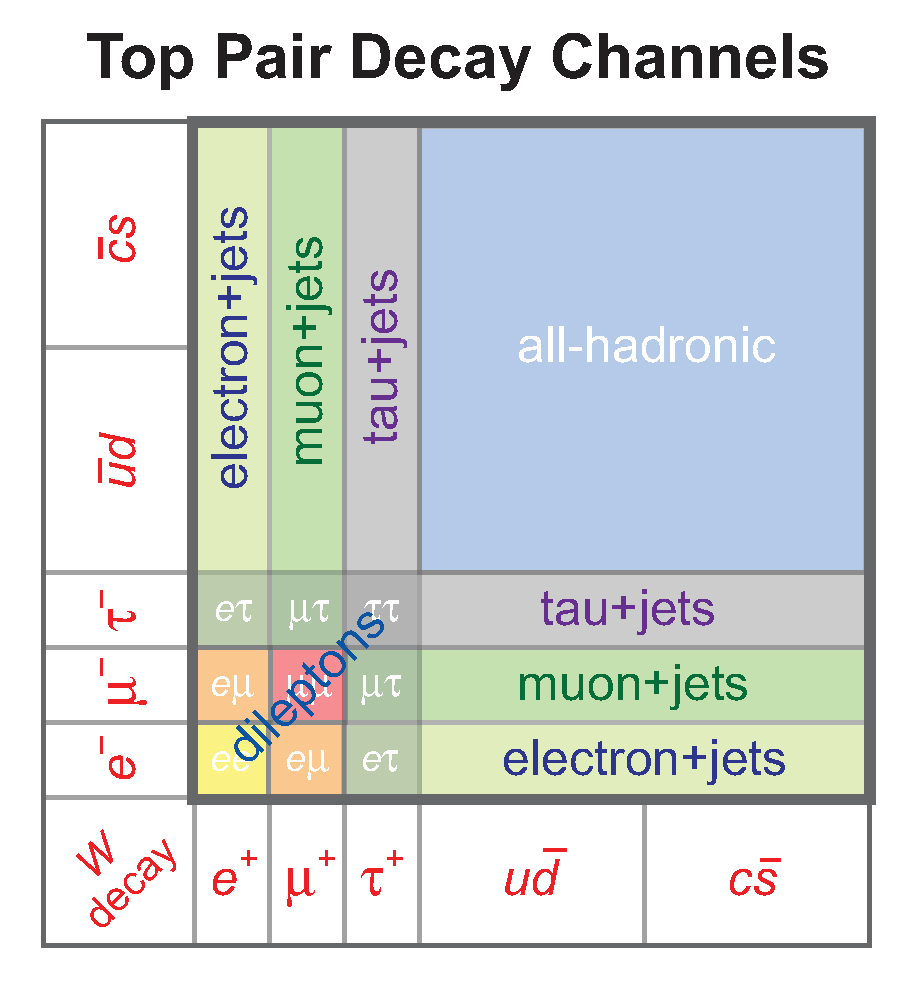
\includegraphics[width=0.40\textwidth]{chapitre5/figs/top_pair_decay_channels.pdf}} \qquad
    \subcaptionbox{\label{fig:top_pair_branching_frac}}[0.45\textwidth]{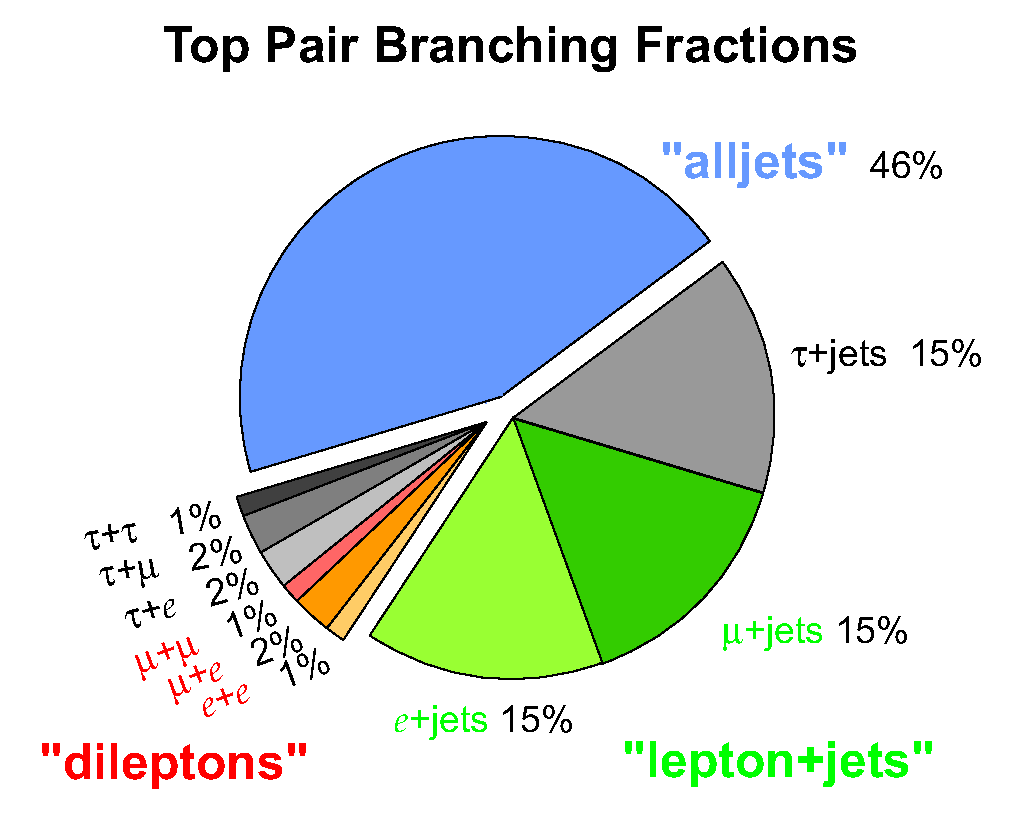
\includegraphics[width=0.45\textwidth]{chapitre5/figs/top_pair_branching_frac.pdf}}
    \caption{Canaux de désintégration d'une paire \ttbar (\subref{fig:top_pair_decay_channels}) et rapports d'embranchements des différents canaux de désintégration d'une paire \ttbar (\subref{fig:top_pair_branching_frac})}
    \label{fig:label}
\end{figure}

Cette classification est résumée \cref{fig:top_pair_decay_channels}. Les rapports d'embranchements associés à chaque canal de désintégration sont résumés \cref{fig:top_pair_branching_frac}. On constate ainsi qu'environ \SI{46}{\%} des paires \ttbar se désintègrent dans le canal tout-hadronique, \tilde\SI{45}{\%} dans le canal semi-leptonique, et \tilde\SI{9}{\%} dans le canal di-leptonique. Les diagrammes de Feynman associés à ces désintégrations sont présentés \cref{fig:top_pair_decay_feynman}.


\begin{figure}[p]
    \centering
    \subcaptionbox{\label{fig:top_pair_decay_dileptonic}}[0.48\textwidth]{\begin{fmfgraph*}(180,150)
        \fmfpen{0.5}
        \fmfleft{t1,i1,i2,t2}
        \fmfright{o1,o2,o3,o4,o5,o6}

        \fmf{gluon}{i1,v1,i2}
        \fmf{gluon}{v1,v2}
        \fmf{fermion,label=\APtop,label.side=left}{v3,v2}
        \fmf{fermion,label=\Ptop,label.side=left}{v2,v4}
        \fmf{boson,label=\PWplus,label.side=left}{v4,v6}
        \fmf{boson,label=\PWminus,label.side=right}{v3,v5}
        \fmf{fermion}{v5,o1}
        \fmf{fermion}{o6,v6}

        \fmffreeze

        \fmf{fermion}{o3,v3}
        \fmf{fermion}{v4,o4}

        \fmf{fermion}{v6,o5}
        \fmf{fermion}{o2,v5}

        \fmflabel{\Pmuon}{o1}
        \fmflabel{\APnum}{o2}

        \fmflabel{\APbottom}{o3}
        \fmflabel{\Pbottom}{o4}

        \fmflabel{\Pnue}{o5}
        \fmflabel{\APelectron}{o6}

        \fmfdot{v1,v2,v3,v4,v5,v6}
    \end{fmfgraph*}}\hfill
    \subcaptionbox{\label{fig:top_pair_decay_semileptonic}}[0.48\textwidth]{\begin{fmfgraph*}(180,150)
        \fmfpen{0.5}
        \fmfleft{t1,i1,i2,t2}
        \fmfright{o1,o2,o3,o4,o5,o6}

        \fmf{gluon}{i1,v1,i2}
        \fmf{gluon}{v1,v2}
        \fmf{fermion,label=\APtop,label.side=left}{v3,v2}
        \fmf{fermion,label=\Ptop,label.side=left}{v2,v4}
        \fmf{boson,label=\PWplus,label.side=left}{v4,v6}
        \fmf{boson,label=\PWminus,label.side=right}{v3,v5}
        \fmf{fermion}{v5,o1}
        \fmf{fermion}{o6,v6}

        \fmffreeze

        \fmf{fermion}{o3,v3}
        \fmf{fermion}{v4,o4}

        \fmf{fermion}{v6,o5}
        \fmf{fermion}{o2,v5}

        \fmflabel{\Pmuon}{o1}
        \fmflabel{\APnum}{o2}

        \fmflabel{\APbottom}{o3}
        \fmflabel{\Pbottom}{o4}

        \fmflabel{\Pquark}{o5}
        \fmflabel{$\APquark^\prime$}{o6}

        \fmfdot{v1,v2,v3,v4,v5,v6}
    \end{fmfgraph*}}\\


    \subcaptionbox{\label{fig:top_pair_decay_hadronic}}[0.48\textwidth]{\begin{fmfgraph*}(180,150)
        \fmfpen{0.5}
        \fmfleft{t1,i1,i2,t2}
        \fmfright{o1,o2,o3,o4,o5,o6}

        \fmf{gluon}{i1,v1,i2}
        \fmf{gluon}{v1,v2}
        \fmf{fermion,label=\APtop,label.side=left}{v3,v2}
        \fmf{fermion,label=\Ptop,label.side=left}{v2,v4}
        \fmf{boson,label=\PWplus,label.side=left}{v4,v6}
        \fmf{boson,label=\PWminus,label.side=right}{v3,v5}
        \fmf{fermion}{v5,o1}
        \fmf{fermion}{o6,v6}

        \fmffreeze

        \fmf{fermion}{o3,v3}
        \fmf{fermion}{v4,o4}

        \fmf{fermion}{v6,o5}
        \fmf{fermion}{o2,v5}

        \fmflabel{$\Pquark^\prime$}{o1}
        \fmflabel{\APquark}{o2}

        \fmflabel{\APbottom}{o3}
        \fmflabel{\Pbottom}{o4}

        \fmflabel{\Pquark}{o5}
        \fmflabel{$\APquark^\prime$}{o6}

        \fmfdot{v1,v2,v3,v4,v5,v6}
    \end{fmfgraph*}}
    \caption{Diagrammes de Feynman de la désintégration d'une paire \ttbar dans le canal di-leptonique (\subref{fig:top_pair_decay_dileptonic}), dans le canal semi-leptonique (\subref{fig:top_pair_decay_semileptonic}), ainsi que dans le canal tout-hadronique (\subref{fig:top_pair_decay_hadronic}).}
    \label{fig:top_pair_decay_feynman}
\end{figure}

\end{fmffile}

\section{Propriétés du quark top}

Découvert en 1995, les propriétés du quark top sont encore assez méconnues. On présente dans cette section un récapitulatif des dernières mesures expérimentales des propriétés du quark top.

\subsection{Masse}

Comme pour les autres particules du Modèle Standard, la masse du quark top est un paramètre libre. Il est néanmoins possible de prédire cette masse grâce aux corrections radiatives lors du calcul de la masse des bosons $W$. Cette masse est mesurée précisément par les expériences du LHC et du Tevatron, et est en excellent accord avec les prédictions théoriques :

\begin{align*}
  m_t^{\text{théorique}} &= 175{,}8 \substack{+2{,}7 \\ -2{,}4}\,\si{\GeV}\ \citep{ewk_fit} \\
  m_t^{\text{Tevatron}} &= 173{,}20 \pm 0{,}51\;\text{(stat.)} \pm 0{,}71\;\text{(syst.)}\;\si{\GeV}\ \citep{CDF:2013jga}\\
  m_t^{\text{LHC}} &= 173{,}34 \pm 0{,}47\;\text{(stat.)} \pm 1{,}34\;\text{(syst.)}\;\si{\GeV}\ \citep{CMS:2013sfa}
\end{align*}

On présente \cref{fig:top_mass_combination} les mesures de la masse du quark top obtenues ATLAS et CMS, en considérant différents états finaux. Le résultat de la combinaison est présenté en bleu, à comparer avec le résultat combiné obtenu au Tevatron en rouge.

\begin{figure}[tbp]
    \centering
    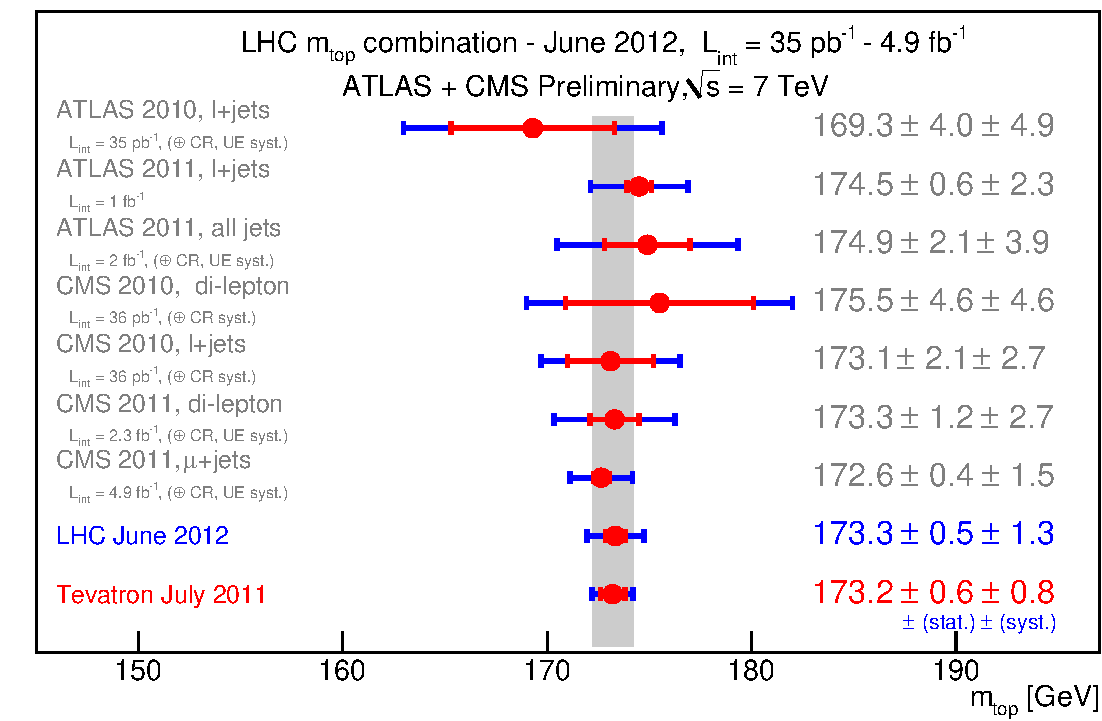
\includegraphics[width=0.70\textwidth]{chapitre5/figs/lhc_top_mass.pdf}
    \caption{Mesure de la masse du quark top grâce aux combinaisons des analyses ATLAS et CMS.}
    \label{fig:top_mass_combination}
\end{figure}

\subsection{Largeur}

La largeur de désintégration du quark top est prédite par le Modèle Standard. Des calculs au NLO donnent
\begin{align*}
  \Gamma_t &= \frac{G_F m_t^3}{8 \pi \sqrt{2}} \, \abs{V_{tb}}^2 \, \left( 1 - \frac{M_W^2}{m_t^2} \right)^2 \left( 1 + 2 \frac{M_W^2}{m_t^2} \right) \left[ 1 - \frac{2 \alpha_s}{3 \pi} \left( \frac{2\pi^2}{3} - \frac{5}{2} \right) \right].
\end{align*}

En utilisant $V_{tb} = 1$, $\alpha_s = \num{0.118}$, $m_t = \SI{173.3}{\GeV}$ et $M_W = \SI{80.4}{\GeV}$, on obtient une largeur $\Gamma_t = \SI{1.27}{\GeV}$, soit un temps de vie $\tau_t = \SI{5.16e-25}{\s}$. Expérimentalement, elle a été déterminée par les expériences D0 et CDF au Tevatron. La valeur la plus précise obtenue à ce jour est $\Gamma_t = 2{,}00 \substack{+0{,}47 \\ -0{,}43}\,\si{\GeV}$ \citep{Abazov:2012vd}, en bon accord avec la valeur théorique.

\subsection{Charge électrique}

Rien ne permet de prouver que la particule découverte au Tevatron est bien le partenaire d'isospin du quark $b$. Un modèle particulier propose en effet un quark de charge $-4/3$ et de masse \tilde \SI{170}{\GeV} comme alternative au quark top du Modèle Standard \citep{PhysRevD.59.091503}.

Afin de déterminer la charge électrique du quark top, on sélectionne des événements \ttbar dans le canal semi-leptonique. Dans le cas du modèle standard, on a
\begin{align*}
  t^{(2/3)} \rightarrow b^{(-1/3)} + W^{(+1)}
\end{align*}
alors que dans le cas d'un quark top exotique ($t_X$), on a
\begin{align*}
  t_X^{(-4/3)} \rightarrow b^{(-1/3)} + W^{(-1)}
\end{align*}
où la charge électrique est spécifiée entre parenthèse. En identifiant la charge du quark $b$ ainsi que celle du lepton (émis lors de la désintégration du boson $W^\pm$), il est possible de déduire la charge du quark top. Des analyses menées par les collaborations ATLAS, CDF et CMS ont permis de confirmer que la charge du quark top découvert est Tevatron est bien de charge $2/3$, avec un niveau de confiance supérieur à \SI{99}{\%} \citep{CMS-PAS-TOP-11-031,Aaltonen:2013sgl,Aad:2013uza}.


\subsection{Hélicité du boson W}

Le top quark se désintègre uniquement par interaction faible, principalement en \Pbottom{}\PW. L'interaction faible ne couplant que les particules d'hélicité gauche, cela limite les états d'hélicité autorisés par le Modèle Standard pour le boson \PW. En effet, au niveau de l'arbre, seul les états d'hélicités gauche et longitudinale sont autorisés. Au NNLO, le Modèle Standard prédit les fractions d'hélicité du boson \PW suivantes \citep{Czarnecki:2010gb} :
\begin{align*}
  F_0 &= \num{0.687 \pm 0.005} \\
  F_G &= \num{0.311 \pm 0.005} \\
  F_D &= \num{0.0017 \pm 0.0001}
\end{align*}

Une déviation dans la mesure de ces fractions d'hélicités serait le signe d'un couplage \Ptop{}\PW{}\Pbottom anormal, et donc un signe de nouvelle physique. Ces fractions ont été mesurées expérimentalement par l'expérience CMS \citep{CMS-PAS-TOP-13-008}. Les valeurs obtenues,
\begin{align*}
  F_0 &= 0{,}659 \pm 0{,}015\;\text{(stat.)} \pm 0{,}023\;\text{(syst.)} \\
  F_G &= 0{,}350 \pm 0{,}010\;\text{(stat.)} \pm 0{,}024\;\text{(syst.)} \\
  F_D &= -0{,}009 \pm 0{,}006\;\text{(stat.)} \pm 0{,}020\;\text{(syst.)}
\end{align*}
sont en parfait accord avec le Modèle Standard.

\subsection{Corrélations de spin}

À cause de son temps de vie très faible, l'information de spin du quark top est directement transmise à ses produits de désintégration. Cette information peut être extraite grâce à l'observation de certaines variables angulaires. Il est alors possible de déterminer expérimentalement la polarisation du spin du quark top, ainsi que les corrélations de spin des paires \ttbar.

Si l'on se concentre la désintégration de paires \ttbar dans le canal di-leptoniques, la différence entre les angles azimutaux des leptons chargés ($\Delta\phi_{\Pleptonplus\Pleptonminus}$) est sensible à la corrélation de spin des paires \ttbar, et peut être mesurée sans reconstruire l'événement \ttbar. La variable $\theta_{\Plepton}$, mesurant l'angle entre du lepton chargé dans le référentiel d'hélicité (relatif à la direction du quark top dans le référentiel de centre de masse), permet d'étudier la polarisation du spin du quark top. Des déviations dans la mesure de ces quantités par rapport aux prédictions du Modèle Standard seraient le signe de la présence de nouvelle physique liée au quark top.

\smallskip

La polarisation $P$ du quark top est donnée par $P = 2A_P$, où l'asymétrie $A_p$ est définie par
\begin{align*}
  A_P &= \frac{N\left( \cos{\left(\theta_{\Plepton}\right)} > 0 \right) - N\left( \cos{\left(\theta_{\Plepton}\right)} < 0 \right)}{N\left( \cos{\left(\theta_{\Plepton}\right)} > 0 \right) + N\left( \cos{\left(\theta_{\Plepton}\right)} < 0 \right)}
\end{align*}

Pour la corrélation de spin des paires \ttbar, la variable
\begin{align*}
  A_{\Delta\phi} &= \frac{ N\left(\Delta\phi_{\Pleptonplus\Pleptonminus} > \frac{\pi}{2} \right) - N\left(\Delta\phi_{\Pleptonplus\Pleptonminus} < \frac{\pi}{2} \right) }{ N\left(\Delta\phi_{\Pleptonplus\Pleptonminus} > \frac{\pi}{2} \right) + N\left(\Delta\phi_{\Pleptonplus\Pleptonminus} < \frac{\pi}{2} \right) }
\end{align*}
fournie une excellente discrimination entre des spins \Ptop et \APtop corrélés ou décorrélés. Les mesures les plus récentes sont fournies par la collaboration CMS, qui trouve des résultats en parfait accord avec les prédictions du Modèle Standard. Ces résultats sont résumés \cref{tab:top_correlation}.

\begin{table}[ht] \centering
\begin{tabular}{@{}cccc@{}} \toprule
Asymétrie & Mesure & Théorie (NLO, corrélé) & Théorie (NLO, décorrélé) \\ \midrule
$A_{\Delta\phi}$ & \num{0.113 \pm 0.017} & $0{,}115 \substack{+0{,}014 \\ -0{,}016}$ & $0{,}210 \substack{+0{,}013 \\ -0{,}008}$ \\
$A_{P}$ & \num{0,005 \pm 0,025} & \multicolumn{2}{c}{\num{0.000 \pm 0.001}} \\ \bottomrule
\end{tabular}
\caption{Comparaison entre les mesures expérimentales et la théorie pour la corrélation de spin de paires \ttbar et la polarisation de spin du quark top. Les prédictions théoriques corrélé et décorrélé n'ont de sens que pour la mesure de la corrélation de spin. Les mesures expérimentales indiquent la présence de corrélation de spin dans les paires \ttbar et l'absence de polarisation de spin.}
\label{tab:top_correlation}
\end{table}

\section{Au-delà du Modèle Standard}

On a déjà vu lors du \cref{chap:sm} que de nombreux arguments laissent penser que le Modèle Standard n'est qu'une théorie effective d'un modèle à plus haute énergie. De nombreux modèles existent ainsi, chacun prédisant de nouvelles particules, forces, dimensions, ... Pour autant, aucun de ces modèles n'a encore été découvert expérimentalement. C'est pour ça que de nombreuses recherches sont actuellement en cours parmi les expériences du LHC afin de tenter de découvrir des signes de nouvelles physiques, ou, le cas échant, de contraindre certains modèles afin d'aider les théoriciens à développer des théories encore plus pertinentes.

Parmi ces modèles, un grand nombres prévoient des phénoménologies où le quark top joue un rôle particulier. En effet, étant la particule fondamentale la plus massive, il est naturel de penser que des nouvelles particules à l'échelle du \si{\TeV} se désintègrent préférentiellement en paires \ttbar. Les travaux réalisés au cours de cette thèse se concentrent sur la recherche de déviations dans le spectre de masse invariante \ttbar ($d\sigma / d\mtt$), déviations pouvant être causées par la production résonante de paire de quark top \emph{via} la désintégration d'une particule exotique. Ces déviations peuvent se présenter sous plusieurs formes, selon la présence ou non d'interférences avec la production du Modèle Standard. Dans le cas le plus simple, elles prennent la forme d'un pic dans le spectre de masse invariante. Des structures plus complexes peuvent aussi être observées, comme la présence d'un pic suivi d'un trou. Ces déviations seront présentées plus en détails dans les \cref{chap:zprime,chap:higgs}, dédiés à la recherche expérimentale de résonances dans le spectre de masse \ttbar.

\medskip

De nombreux modèles prédisent des particules se désintégrant en paire de quark top. On présente ci-dessous une description succincte des modèles les plus prometteurs, classés selon le spin des particules exotiques. On présente \cref{tab:summary_bsm} un résumé des modèles de nouvelle physique, classé selon le spin des particules prédites, leur parité sous la symétrie CP, et leur représentation sous $SU(3)_c$.

\subsection{Le Modèle Standard et les résonances \ttbar}

À la différence des autres quarks, le quark top n'existe pas sous forme d'état lié \ttbar, son temps de vie étant trop faible devant le temps moyen d'hadronisation. La seule production résonante \ttbar prédite par le Modèle Standard est \emph{via} la désintégration d'un boson de Higgs massif. La récente découverte d'un boson compatible avec le boson de Higgs, de masse \tilde\SI{125}{\GeV}, exclu cette possibilité puisque $m_{\PHiggs} < 2\,m_{\Ptop}$. Il n'existe donc aucune prédiction de résonance \ttbar par le Modèle Standard. Toute déviation dans le spectre de masse \ttbar serait ainsi la preuve de l'existence de nouvelle physique.

\subsection{Modèles à deux doublets de Higgs (2HDM)}